\documentclass[xcolor=dvipsnames,10pt,aspectratio=169]{beamer}
%\documentclass[xcolor=dvipsnames,10pt]{beamer}
\usepackage{etex}
\usepackage{pgf,pgfarrows,pgfnodes,pgfautomata,pgfheaps,pgfshade}
\usepackage[absolute,overlay]{textpos} 
%\usepackage{algorithm}
\usepackage{amsmath,amssymb}
\usepackage[utf8]{inputenc} 
\usepackage{colortbl}
\usepackage{graphicx} 
\usepackage[brazil]{babel}
\usepackage{tabularx} 
\usepackage{multirow}
\usepackage{booktabs}
\usepackage{listings}
\usepackage{multimedia}
\usepackage{animate}
\usepackage{xcolor}
\usepackage{array}
\usepackage{longtable}
\usepackage{makecell}
\usepackage{caption}
\usetheme{Madrid} 

\lstset{ %
%	backgroundcolor=\color{white},   % choose the background color; you must add \usepackage{color} or \usepackage{xcolor}
%	basicstyle=\footnotesize,        % the size of the fonts that are used for the code
	basicstyle=\scriptsize,        % the size of the fonts that are used for the code
	breakatwhitespace=false,         % sets if automatic breaks should only happen at whitespace
	breaklines=true,                 % sets automatic line breaking
	captionpos=t,                    % sets the caption-position to bottom
	commentstyle=\color{mygreen},    % comment style
	deletekeywords={...},            % if you want to delete keywords from the given language
	escapeinside={\%*}{*)},          % if you want to add LaTeX within your code
	extendedchars=true,              % lets you use non-ASCII characters; for 8-bits encodings only, does not work with UTF-8
%	frame=single,                    % adds a frame around the code
	keepspaces=true,                 % keeps spaces in text, useful for keeping indentation of code (possibly needs columns=flexible)
	keywordstyle=\color{blue},       % keyword style
%	language=make,                 % the language of the code
	morekeywords={*,...},            % if you want to add more keywords to the set
%	numbers=left,                    % where to put the line-numbers; possible values are (none, left, right)
%	numbersep=5pt,                   % how far the line-numbers are from the code
	numberstyle=\tiny\color{mygray}, % the style that is used for the line-numbers
	rulecolor=\color{black},         % if not set, the frame-color may be changed on line-breaks within not-black text (e.g. comments (green here))
	showspaces=false,                % show spaces everywhere adding particular underscores; it overrides 'showstringspaces'
	showstringspaces=false,          % underline spaces within strings only
	showtabs=false,                  % show tabs within strings adding particular underscores
	stepnumber=2,                    % the step between two line-numbers. If it's 1, each line will be numbered
}

\definecolor{mygreen}{rgb}{0,0.6,0}
\definecolor{mygray}{rgb}{0.5,0.5,0.5}
\definecolor{mymauve}{rgb}{0.58,0,0.82}

\usecolortheme{beaver}
\newcommand{\ul}{\underline}
\setbeamertemplate{footline}{\scriptsize{\vspace*{0.3cm}\hspace*{15cm}\insertframenumber\,/\,\inserttotalframenumber}}
\setbeamertemplate{caption}[numbered]
\setbeamerfont{caption}{size=\fontsize{8}{5}}

\setbeamercolor{block title}{	bg=Sepia , fg = White}
\setbeamercolor{block body}{bg=Brown!15, fg=Sepia }
\setbeamercolor{item projected}{bg=Sepia, fg=White}
\setbeamercolor{number projected}{bg = Black}

%declara as imagens usadas no layout do slide
%\pgfdeclareimage[height=0.8cm]{mflab}{figuras/logo_mflab_transparente.png}
%\pgfdeclareimage[height=1.0cm]{logoufu}{figuras/logo_ufu.jpg}
%\pgfdeclareimage[height=1.0cm]{petro}{figuras/petrobras_2.png}

%posiciona o logotipo do MFLab
\setlength{\TPHorizModule}{1mm}
\setlength{\TPVertModule}{1mm}
\newcommand{\placelogomflab} 
{ 
	\begin{textblock}{13}(150.0,0.0)
		\pgfuseimage{mflab} 
	\end{textblock} 
	
% 	\begin{textblock}{13}(128.0,1.0)
% 		\pgfuseimage{logoufu} 
% 	\end{textblock} 
	
	\begin{textblock}{13}(150.0,70.0)
		\pgfuseimage{petro} 
	\end{textblock} 
}
%posiciona o logotipo do MFLab
\setlength{\TPHorizModule}{1mm}
\setlength{\TPVertModule}{1mm}
\newcommand{\placelogo} 
{ 
	\begin{textblock}{13}(150.0,0.0)
		\pgfuseimage{mflab} 
	\end{textblock} 
	
% 	\begin{textblock}{13}(128.0,1.0)
% 		\pgfuseimage{logoufu} 
% 	\end{textblock} 
	
	\begin{textblock}{13}(0.0,80.0)
		\pgfuseimage{petro} 
	\end{textblock} 
}

% \setlength{\TPHorizModule}{1mm}
% \setlength{\TPVertModule}{1mm}
% \newcommand{\placelogomflab_titulo} 
% { 
% 	\begin{textblock}{13}(150.0,0.0)
% 		\pgfuseimage{mflab} 
% 	\end{textblock} 
% 	
% 	\begin{textblock}{13}(0.0,0.0)
% 		\pgfuseimage{lmest} 
% 	\end{textblock} 
% 	
% % 	\begin{textblock}{13}(128.0,1.0)
% % 		\pgfuseimage{logoufu} 
% % 	\end{textblock} 
% 	
% 	\begin{textblock}{13}(75.0,80.0)
% 		\pgfuseimage{petro} 
% 	\end{textblock} 
% }



%insere o logotipo da ufu em todos os slides
% \logo{
\includegraphics[height=0.8cm]{figuras/layout_slide/petrobras.png}}

\title{Projeto Statera: Um problema de equilíbrio e controle}

\author{ Felipe J. O. Ribeiro \\ \and \\ Orientador: Prof. Alexandre Zuquete Guarato}

%\date{\tiny{02 de dezembro de 2015}}
\date{\tiny{\today}}
% \newcolumntype{M}[1]{>{\raggedright\arraybackslash}b{#1}}
% \newcolumntype{N}{@{}m{0pt}@{}}	
% \newcolumntype{M}{>{\begin{minipage}[b]{3cm}\raggedright{}}c<{\end{minipage}\minrowheight}}
% \setlength\extrarowheight{5pt}
\newcolumntype{C}[1]{>{\centering\let\newline\\\arraybackslash\hspace{0pt}}m{#1}}


\begin{document}

	\begin{frame}
		\frametitle 
		{ \vfill
			\centering
			{
			\small{Universidade Federal de Uberlândia}\\
%			\small{Programa de Pós-Graduação em Engenharia Mecânica}\\
			\small{Laboratório de Mecânica dos Fluidos}\\
			}
		}
		\maketitle
	\end{frame}

	\section<presentation>*{Sumário}
	
		\begin{frame}
			\frametitle{Sumário} 
			{\scriptsize \tableofcontents}
		\end{frame}

		\AtBeginSection[]
		{
		 \begin{frame}<beamer>
		  \frametitle{Sumário}
		  {\scriptsize \tableofcontents[current,currentsection]}
		 \end{frame}
		}

		\AtBeginSubsection[]
		{
		 \begin{frame}<beamer>
		  \frametitle{Sumário}
		  {\scriptsize \tableofcontents[current,currentsubsection]}
		 \end{frame}
		}





	\section{Proposta}
	
	
	
	
	
		\begin{frame}
			\frametitle{Conceito}
						\begin{tabular}{c c}
							{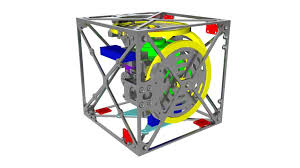
\includegraphics[trim=0.0cm 0.0cm 0.0cm 0.0cm,clip=true,height=0.5\textheight]{imagens/download}}&{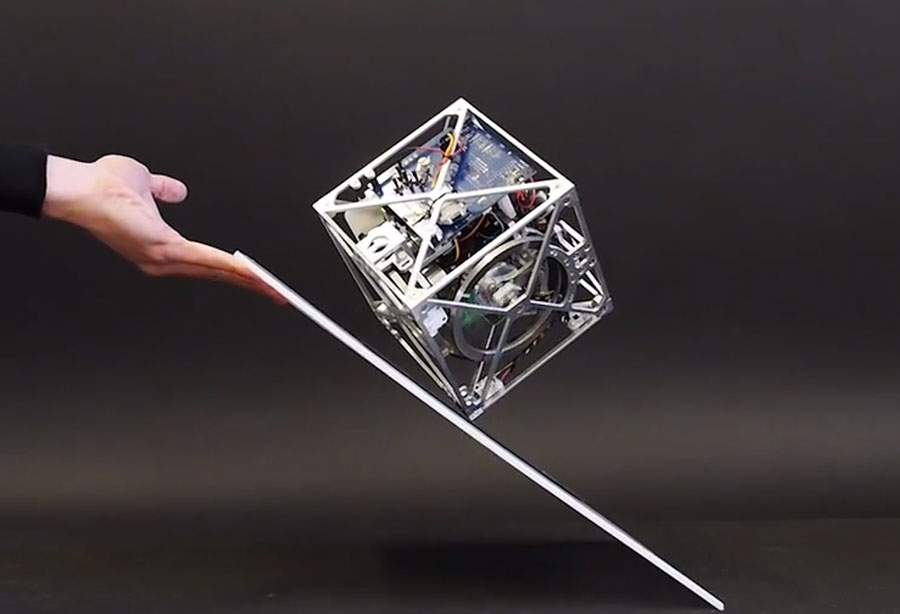
\includegraphics[trim=0.0cm 0.0cm 0.0cm 0.0cm,clip=true,height=0.4\textheight]{imagens/new_cubli}}\\
					\end{tabular}
		\end{frame}
	
	
	
	
	
	\section{Paços de um projeto}
		
		
		
		
		
		\begin{frame}
			\frametitle{Desenvolvimento de primeiro protótipo}
			\centering
			\begin{tabular}{c c}
				{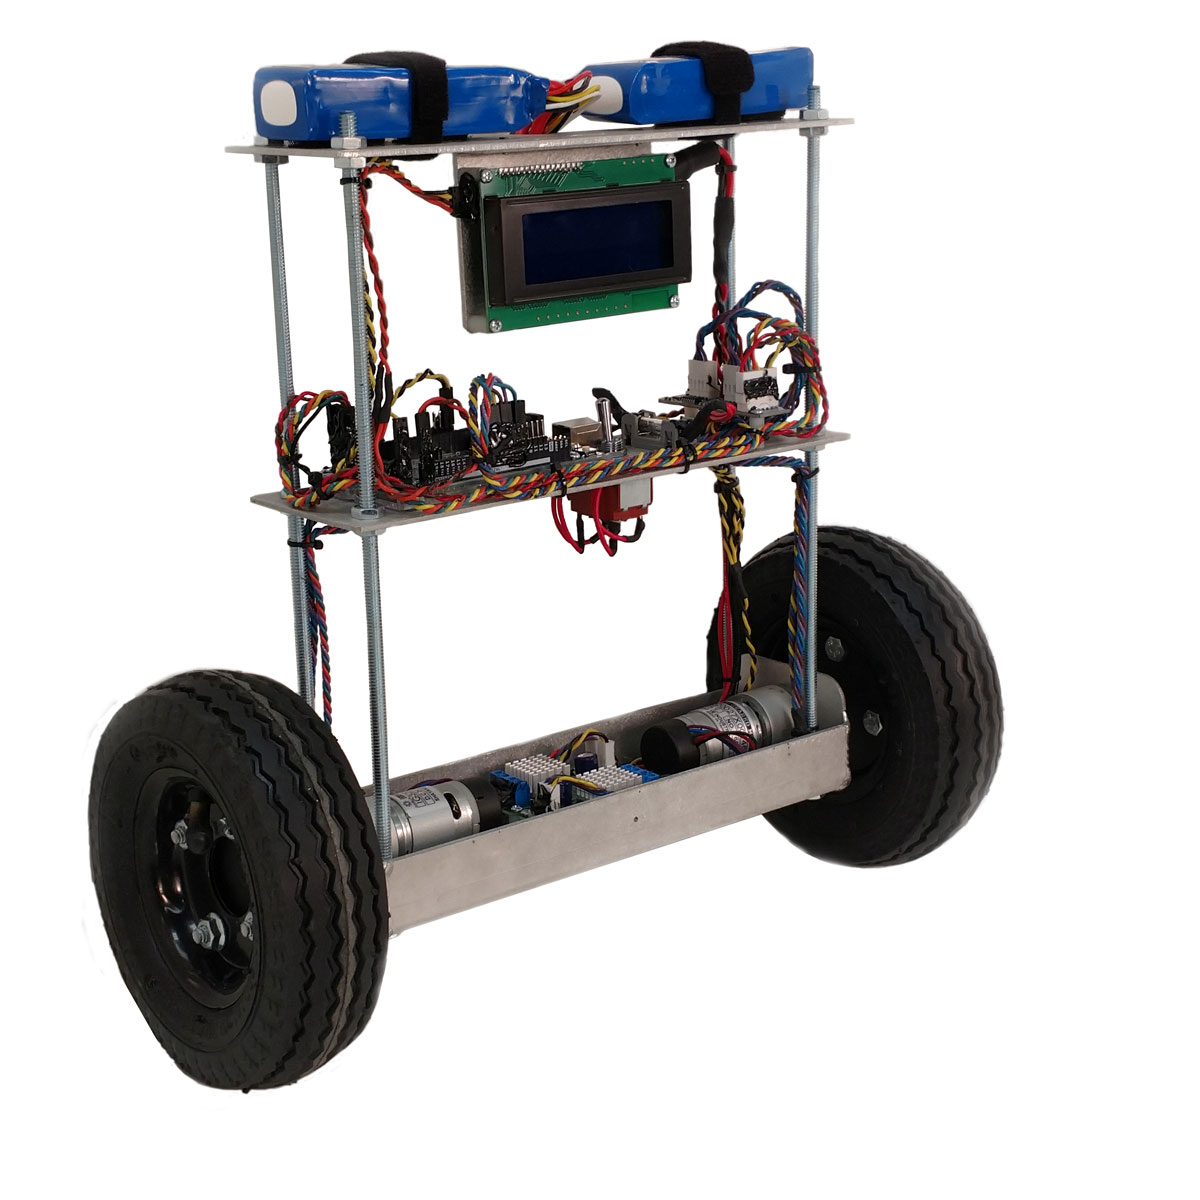
\includegraphics[trim=0.0cm 0.0cm 0.0cm 0.0cm,clip=true,height=0.5\textheight]{imagens/ola}}&{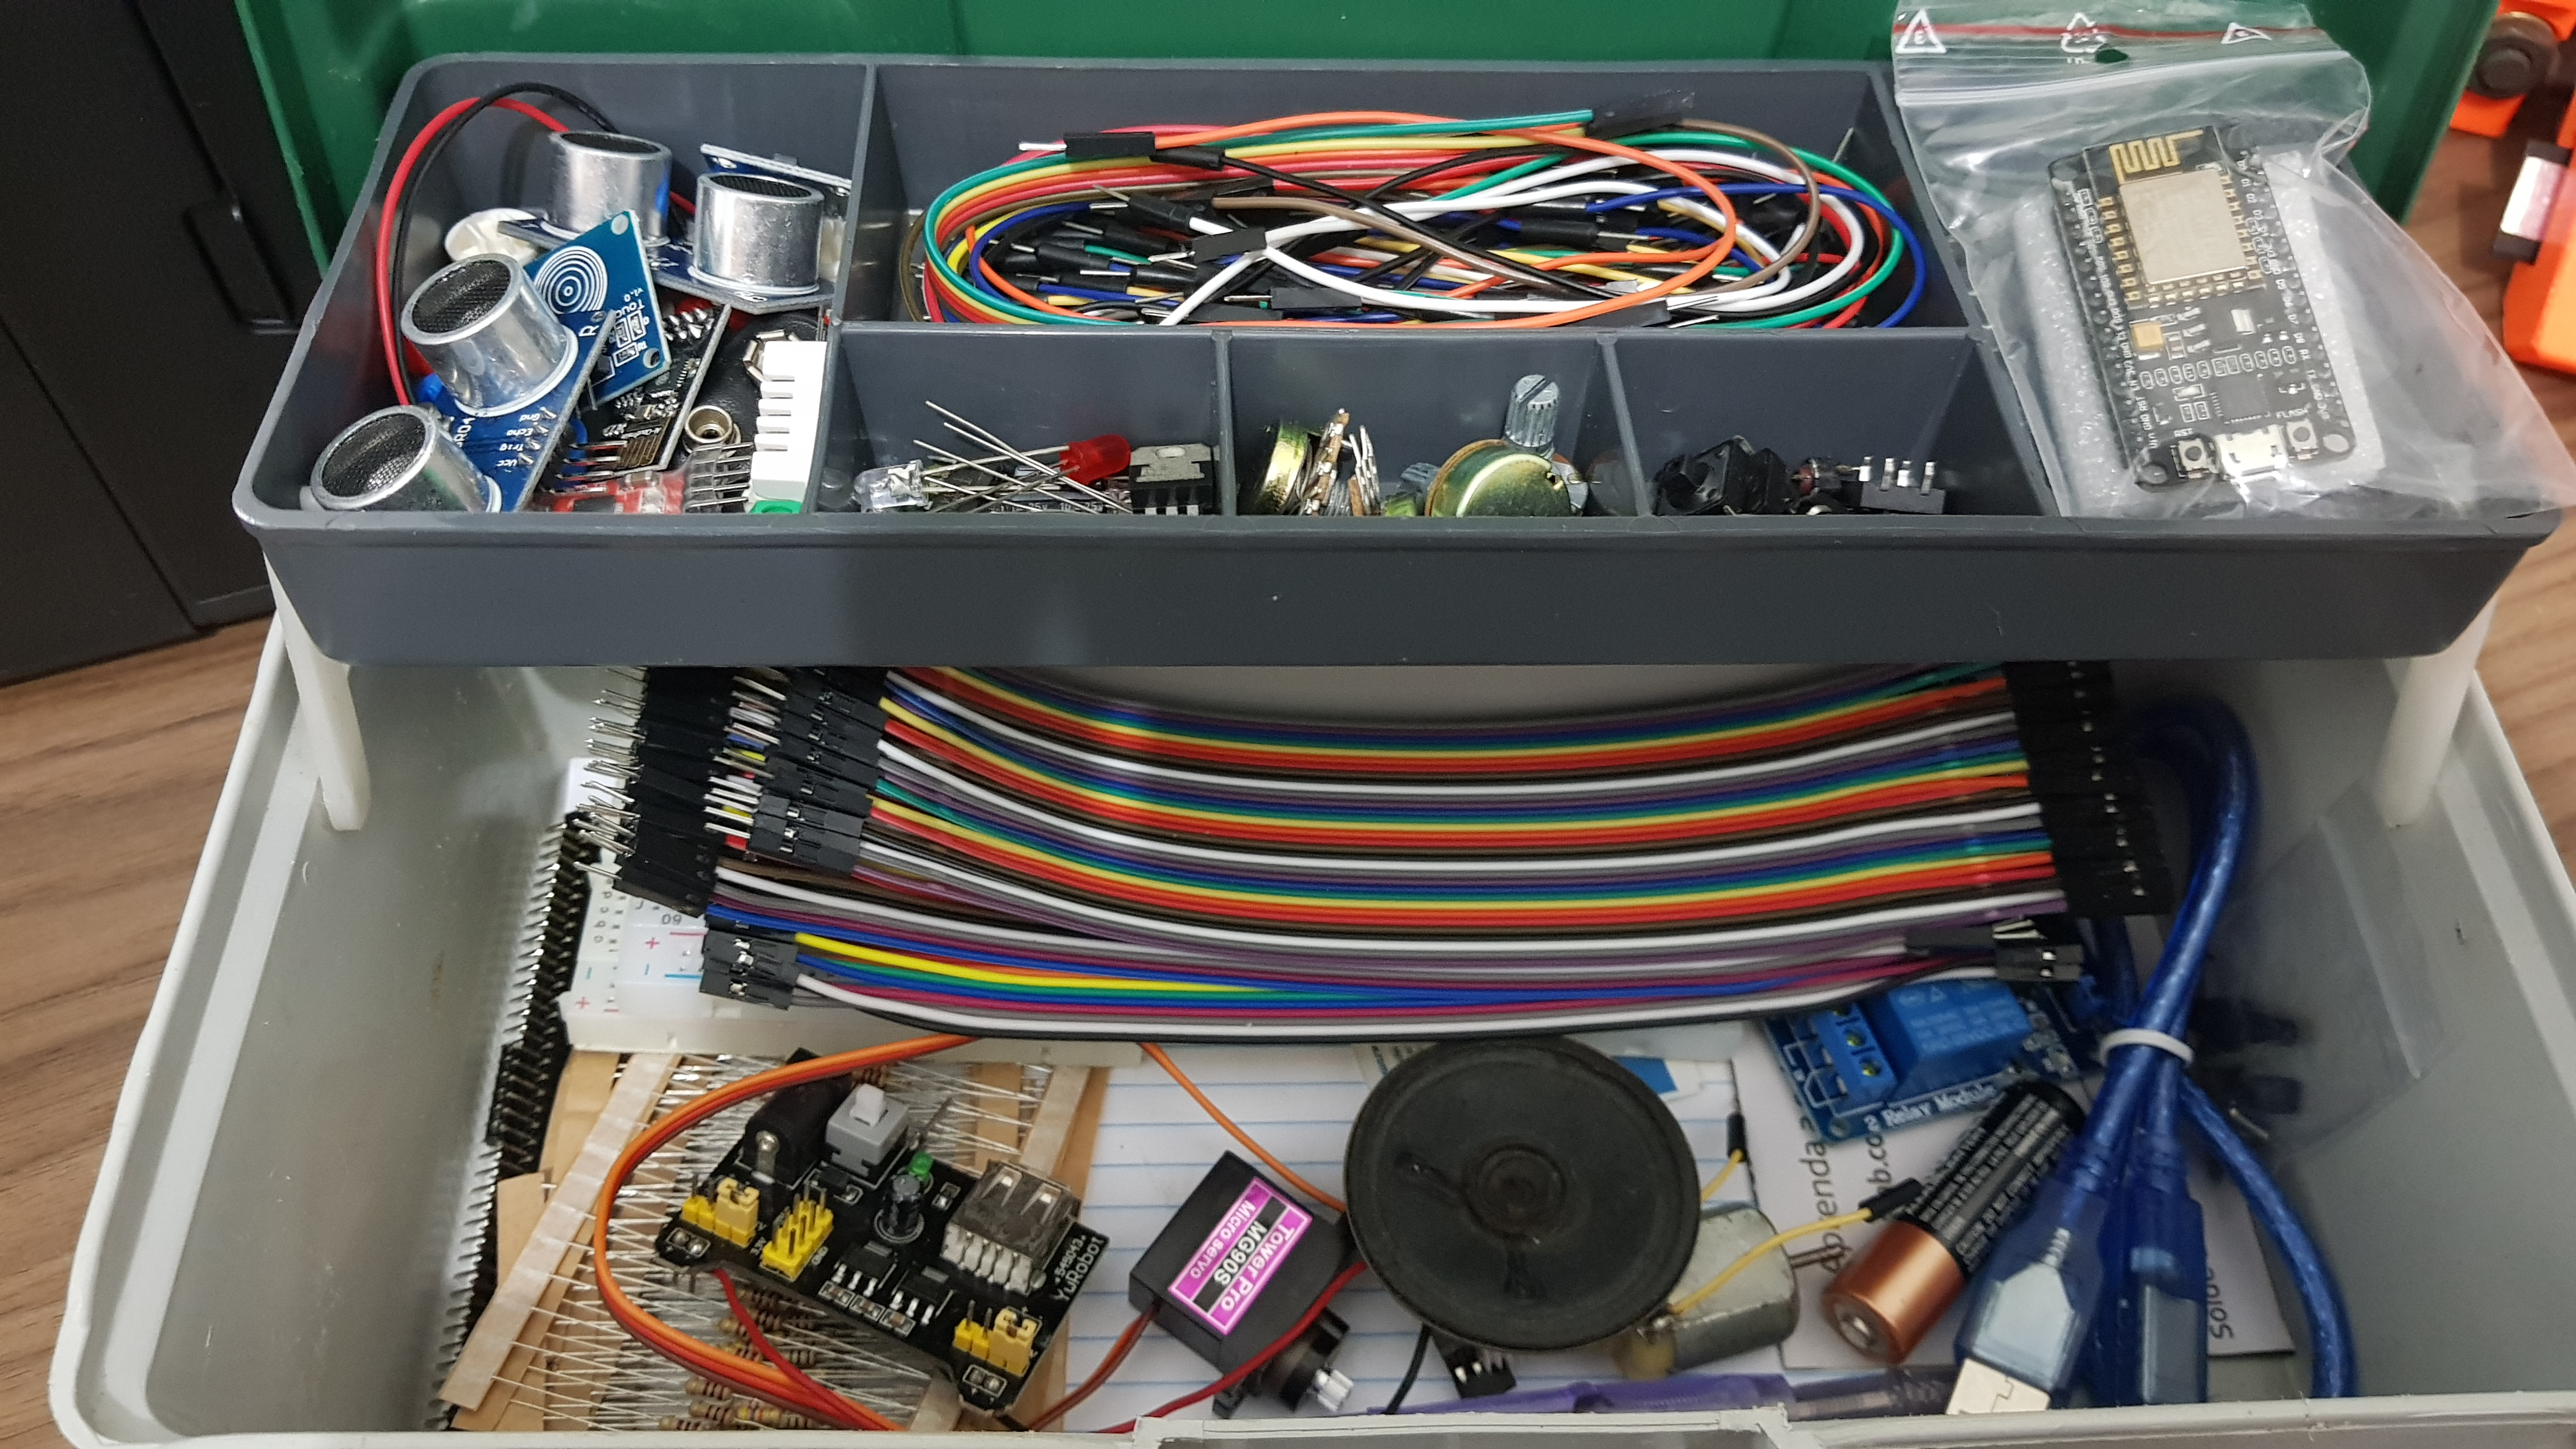
\includegraphics[trim=0.0cm 0.0cm 0.0cm 0.0cm,clip=true,height=0.4\textheight]{imagens/oi}}\\
			\end{tabular}
		\end{frame}





		\begin{frame}
			\frametitle{Modelo final}
			\centering
			{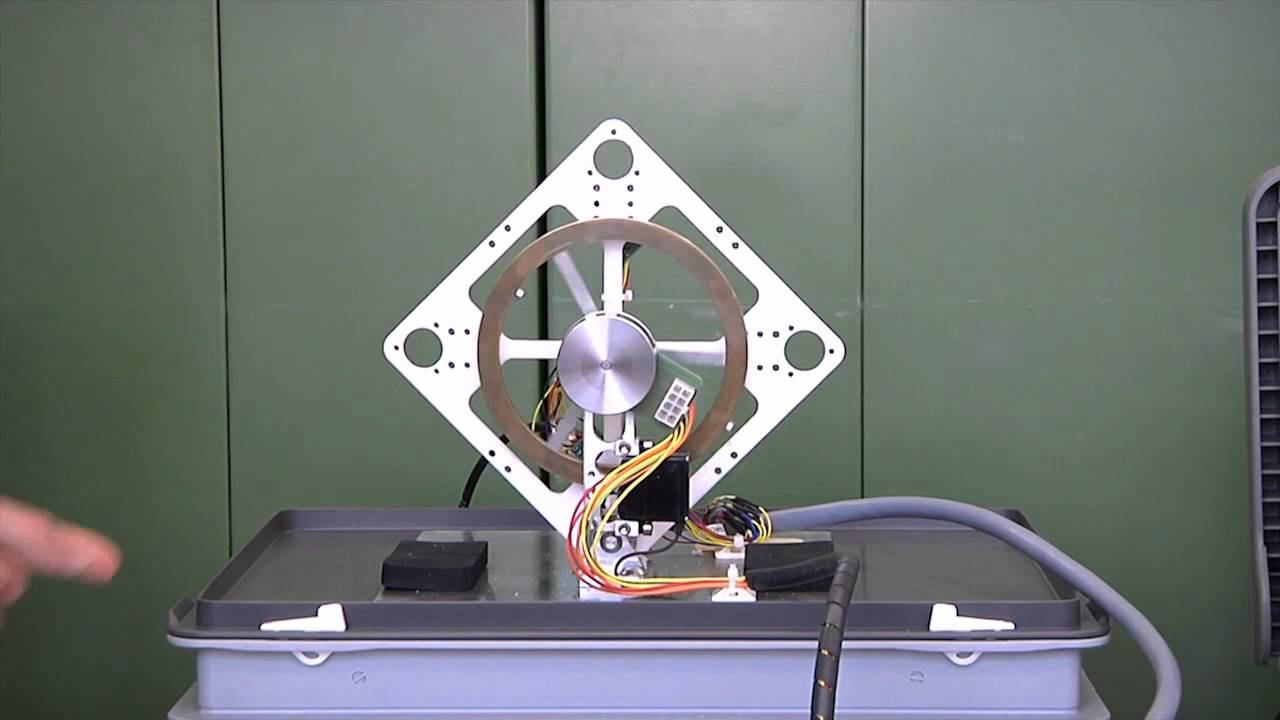
\includegraphics[width=0.6\textwidth]{imagens/maxresdefault}}
		\end{frame}
		
		
		\begin{frame}
        \frametitle{Visão geral}
         \centering
        {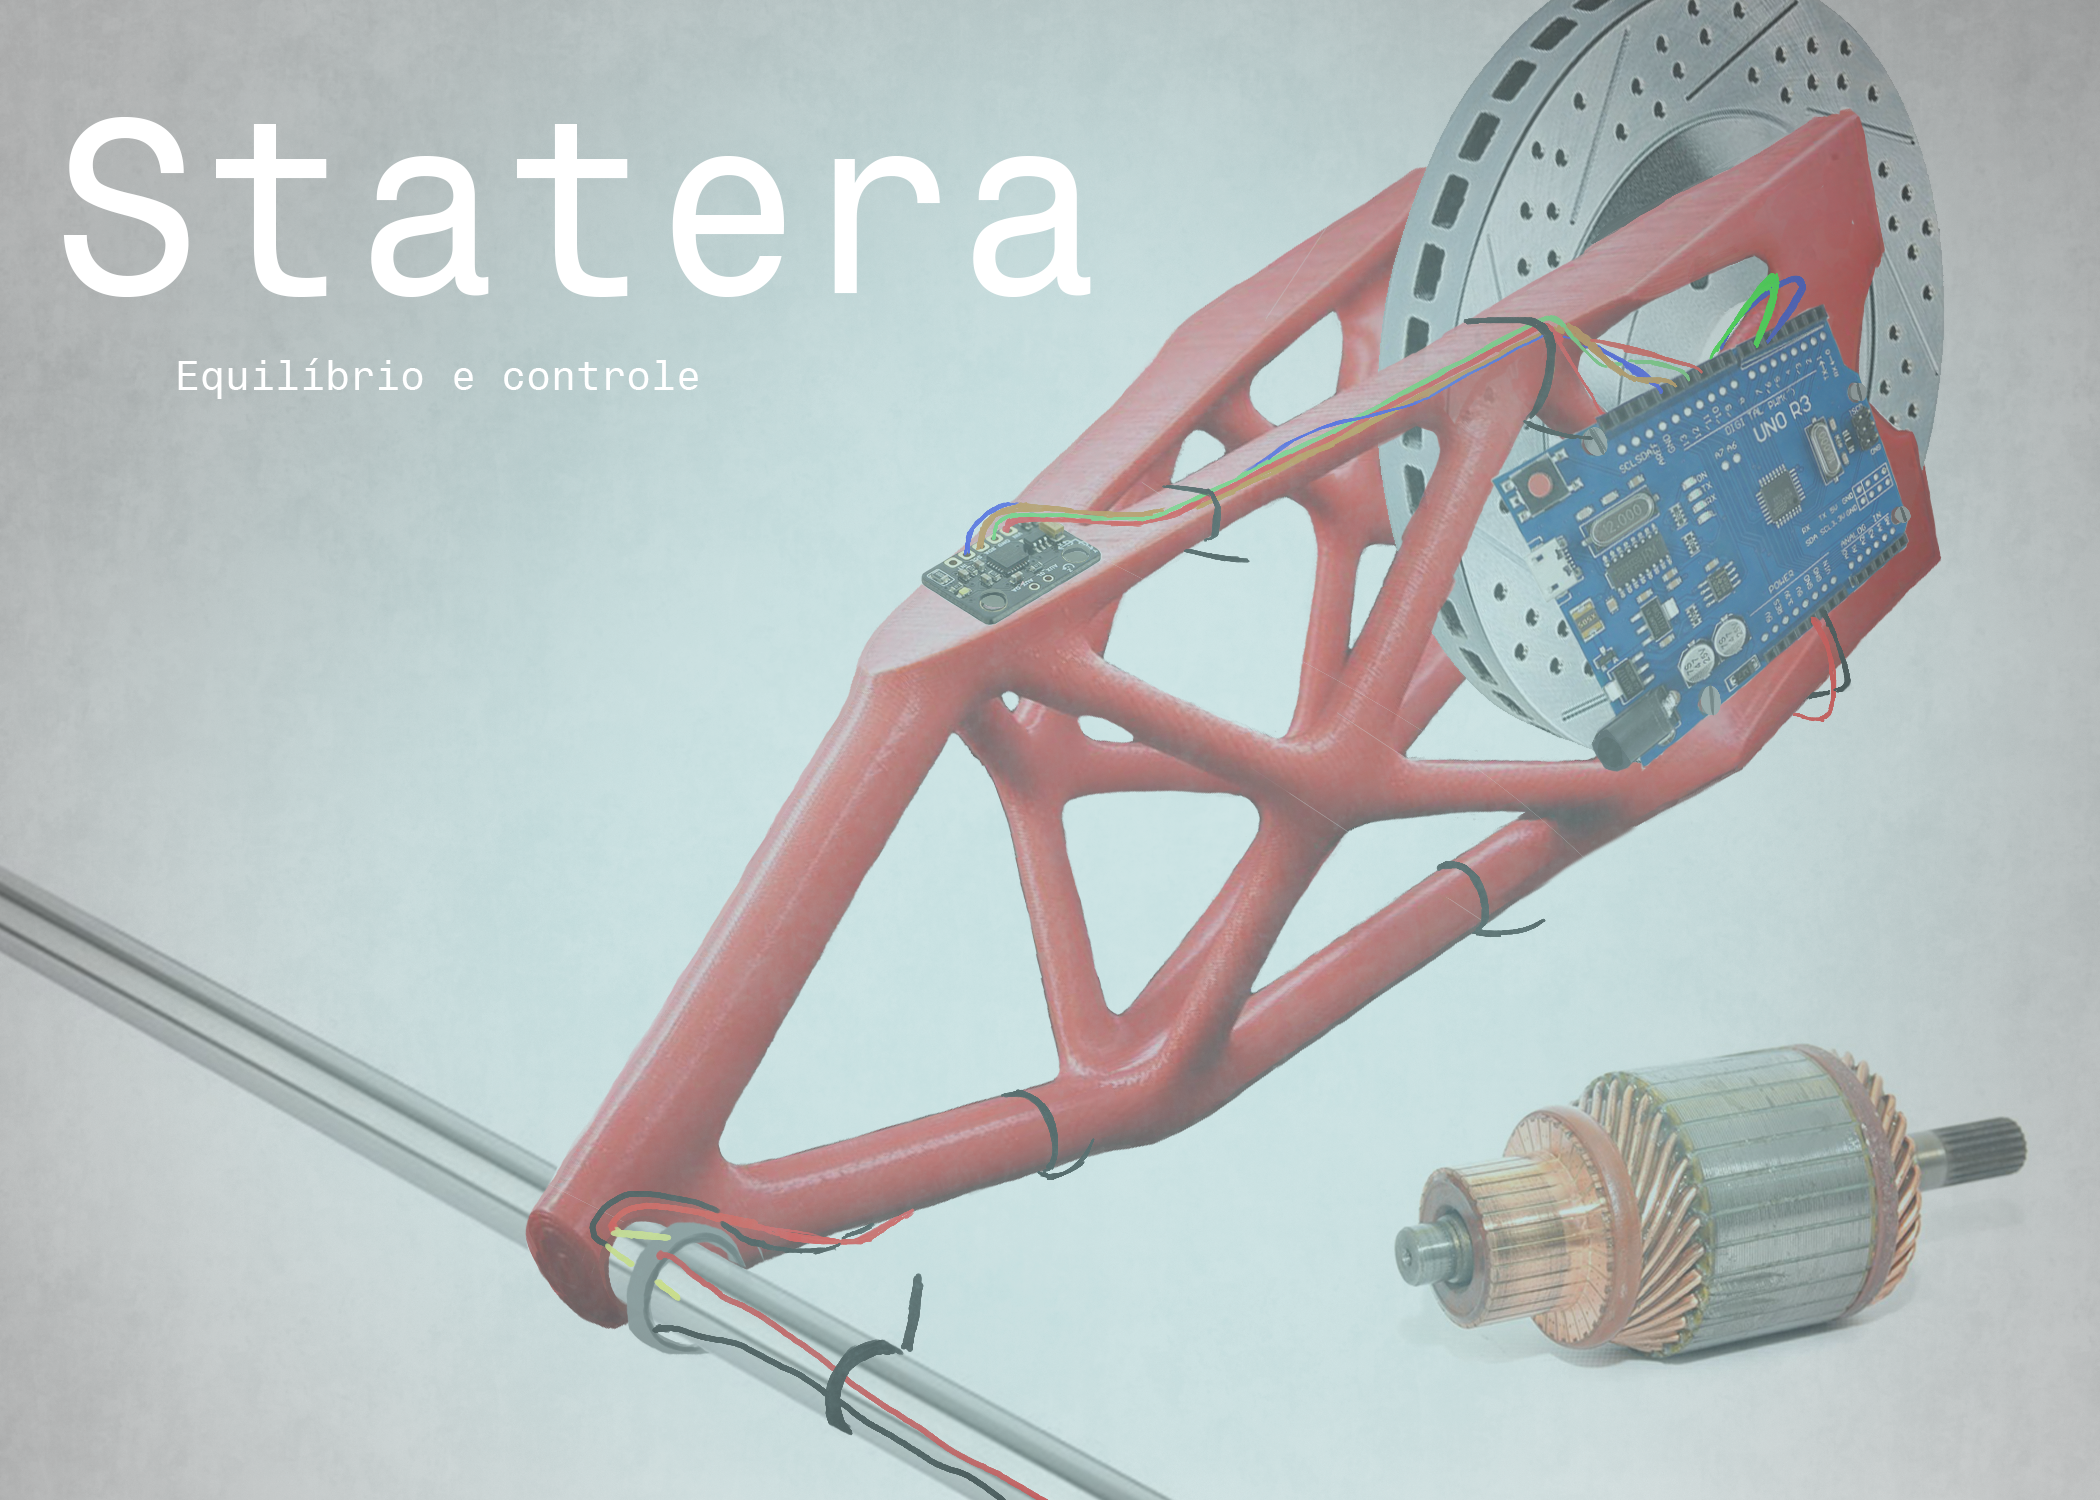
\includegraphics[width=0.6\textwidth]{imagens/visaogeral.png}}
        \end{frame}
		
		
		
			\section{Visão}
			
			\begin{frame}
						\frametitle{Pontos de interesse e possíveis abordagens}
						
						\flushleft
						\textbf{Tópicos:}\\
						$\bullet$ Criação de modelos de resposta ao estímulo externo.\\
						\quad	$\longrightarrow$ Meta-modelagem\\
						\quad	$\longrightarrow$ Algoritmo evolutivo\\
						\quad   $\longrightarrow$ Desenvolvimento algébrico dedutivo de um modelo físico\\
			
						\textbf{Objetivo:}\\
						$\bullet$ Um modelo que tenha sucesso em equilibrar a viga de forma ativa e automática.\\
			
			
			\end{frame}
		
						\begin{frame}
			\frametitle{Agradecimentos}
			\fontsize{44pt}{7.2}\selectfont
			\begin{center}
				Obrigado.
			\end{center}
		\end{frame}
			
			
		
\end{document}




		



%%%%%%%%%%%%%%%%%%%%%%%%%%%%%%%%%%%%%%% Exemplo de formatação de imagens		
%		\begin{frame}
%			\frametitle{Adição de fronteiras extras}
%			\begin{tabular}{c c}
%				
%				{\includegraphics[trim=0.0cm 0.0cm 0.0cm 0.0cm,clip=true,loop,height=0.5\textheight]{figuras/filtration_depois.png}}&{\includegraphics[trim=0.0cm 0.0cm 0.0cm 0.0cm,clip=true,loop,height=0.4\textheight]{figuras/filtration_depois_zoom.png}}\\
%				
%			\end{tabular}
%			
%		\end{frame}




%%%%%%%%%%%%%%%%%%%%%%%%%%%%%%%%%%%%%% Exemplo de formatação de imagens		
%		\begin{frame}
%			\frametitle{Agora}
%			\centering
%			\begin{tabular}{c}
%				
%				{\includegraphics[trim=0.00cm 2.0cm 0.0cm 2.0cm,clip=true,loop,width=0.9\textwidth]{figuras/t_x_51f.png}}\\{\includegraphics[trim=0.01cm 0.0cm 0.01cm 0.0cm,clip=true,loop,width=0.9\textwidth]{figuras/t_x_51999.png}}\\{\includegraphics[trim=0.01cm 0.0cm 0.01cm 0.0cm,clip=true,loop,width=0.9\textwidth]{figuras/t_x_51999g.png}}\\{\includegraphics[trim=0.01cm 0.0cm 0.01cm 0.0cm,clip=true,loop,width=0.9\textwidth]{figuras/t_x_51999y.png}}\\{\includegraphics[trim=0.01cm 0.0cm 0.01cm 0.0cm,clip=true,loop,width=0.9\textwidth]{figuras/t_x_51999b.png}}
%				
%			\end{tabular}
%			
%		\end{frame}





%%%%%%%%%%%%%%%%%%%%%%%%%%%%%%%%%%%%%  Formatação de equações:		
%		\begin{frame}
%			\frametitle{Newton-Raphson}
%			
%			\flushleft
%			Método de interface com jacobiano composto:
%			
%			\centering
%			\begin{equation}\label{forte_eqNewton}
%			K(D+\Delta D) \approx K(D)+\Delta D \, J(D)
%			\end{equation}
%			\begin{equation}\label{forte_eqNewton2}
%			K(D) =  Estrutura(Fluido(D))-D =  0
%			\end{equation}
%			\begin{equation}\label{forte_eqNewton3}
%			J(D) =  Estrutura'(Fluido(D)) \, Fluido'(D)-I
%			\end{equation}
%			\begin{equation}\label{forte_eqNewton4}
%			Fluido(D): \mathbb{R}^{n} \to \mathbb{R}^{m}
%			\end{equation}
%			
%			\flushleft
%			$Fluido'(D)$ é de tamanho $m x n$
%			
%			\centering
%			
%			\begin{equation}\label{forte_eqNewton5}
%			Estrutura(F): \mathbb{R}^{m} \to \mathbb{R}^{n}
%			\end{equation}
%			
%			\flushleft
%			$Estrutura'(F)$ é de tamanho $n x m$\\
%			$Estrutura'(Fluido(D)) \, Fluido'(D)$ e $I$ é de tamanho $n x n$
%		\end{frame}




%%%%%%%%%%%%%%%%%%%%%%%%%%%%%%%%%%%%%%%%%%% Vários exemplos de formatação textual:		


%		\begin{frame}
%			\frametitle{Conveniência do método de Multi Direct Forcing}
%			
%			\flushleft
%			\textbf{Fraco:}\\
%			$\bullet$ Predição da velocidade.\\
%			$\bullet$ MDF. (Imposição da condição de dirichlet na interface e cálculo da força)\\
%			$\bullet$ Estrutura.\\
%			$\bullet$ Poisson.\\
%			$\bullet$ Correção de velocidade e pressão.\\ \\
%
%			\textbf{Forte:}\\
%			$\bullet$ Predição da velocidade.\\
%			while \\
%			\quad	$\longrightarrow$ MDF.\\
%			\quad	$\longrightarrow$ Estrutura.\\
%			end\\
%			$\bullet$ Poisson.\\
%			$\bullet$ Correção de velocidade e pressão.\\
%
%		\end{frame}

		

%		
%%%%%%%%%%%%%%%%%%%%%%%%%%%%%%%%%  Modelo duas fotos lado a lado:


%		\begin{frame}
%		\frametitle{Limite do fraco}
%			ct=121
%			mi=200
%			\begin{tabular}{c c}
%			{\includegraphics[width=0.45\linewidth]{../../simulacoes_Estudo_dirigido2/fraco_mi_200_0_15_ct141/figuras/estrutura/vel_151}}&
%		   {\includegraphics[width=0.45\linewidth]{../../simulacoes_Estudo_dirigido2/fraco_mi_200_0_15_ct141/figuras/estrutura/vel_251}}\\
%		   {(a) Velocidade em linha centro da estrutura} & {(b) Velocidade transversal centro da estrutura}
%		\end{tabular}
%		\end{frame}



%%%%%%%%%%%%%%%%%%%%%%%%%%%%%%%%%%  Modelo tabela :

%		\begin{frame}
%			\frametitle{Comparação número de iterações}
%			\begin{tabular}{c c c c}
%				\hline
%				Método & Mínimo     &    Máximo &  Média\\ \hline
%				FPI MDF variável & 8     &    101 &  8.9764764764764760\\
%				FPI MDF fixo & 8     &     11 &  8.9099099099099099\\
%				QN Primeiro método de Broyden MDF variável & 18    &     101 &  18.281281281281281 \\ \hline
%			\end{tabular}
%		\end{frame}	




